\section{ Threat Model }

    The goal of this work is to completely isolate software modules that share
    hardware with one another. Virtual memory, processes, and machine 
    virtualization provide isolation through explicit channels. However, these 
    approaches to isolate software do not address timing channels that leverage 
    shared hardware. Interference in microarchitectural components can still 
    leak sensitive information.
    
    This is problematic for hardware/software architectures that rely on 
    software isolation to permit distrusting parties to share hardware. One 
    such example is platform as a service cloud computing wherein a hypervisor 
    controls virtual machines (VMs)
    which are leased to end-users. In this model, it is possible for a 
    malicious user to circumvent the isolation provided by virtualization and 
    extract secrets from a co-resident VM  through timing channels.

    Our approach to controlling timing channels is to group software modules 
    (such as VMs) into a hardware/software architecture primitive called a 
    timing compartment. A small, software trusted computing
    base sets up these timing compartments and initializes the hardware to 
    track actions performed on behalf of these timing compartments at the 
    hardware level. Then, the hardware architecture controls how the timing 
    compartments use shared resources to eliminate interference and provide 
    strong timing channel isolation. Timing compartments are described in 
    further detail in the following section. Intuitively, a single timing 
    compartment contains only software modules that trust each other (such as 
    all the VMs on a machine owned by the same user), however, timing channel 
    leakage between modules in different timing compartments must be 
    controlled.

    \begin{figure}
        \begin{center}
            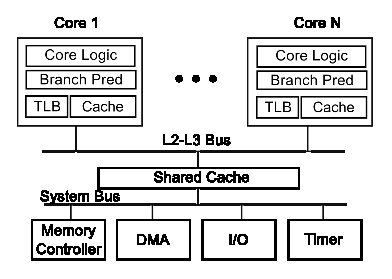
\includegraphics[width=3in]{figs/baseline.eps}
            \caption{The timing-channel vulnerable baseline architecture.}
            \label{fig:baseline}
        \end{center}
    \end{figure}

    Figure \ref{fig:baseline} shows a general hardware/software architecture on 
    which we base our threat model. The hardware architecture has multiple 
    cores, each with private resources such as a branch predictor, one or more 
    private caches, a TLB, and the core logic. Each processor is connected to a 
    shared cache through an on-chip network. The multicore processor is 
    connected to the main memory and a DMA module through the system bus. 

    The hardware is concurrently shared by multiple timing compartments. As 
    shown in Figure \ref{fig:baseline}, it is possible for a timing compartment 
    to have multiple software modules which may be allocated to different 
    cores. It is also possible for timing compartments to be time multiplexed 
    on the same core (e.g.  by context switching VMs), but it is not possible 
    for timing compartments to execute concurrently on the same core (e.g.  
    through SMT).
    
    The software monitor in Figure \ref{fig:baseline} is responsible for 
    setting up and managing the timing compartments and initializing the 
    hardware mechanisms that control them. This software monitor must be 
    trusted as each timing compartment must rely on it. Similarly, the hardware 
    itself is trusted and attacks that require physical possession of the 
    hardware are not addressed by this work.
